%==============================================================================
%  PART 4 --- PREDICTION & CONCLUSIONS (Task 3)
%  Chapters: Outcome Prediction | Discussion | Limitations & Future Work |
%            Conclusions
%==============================================================================

\chapter{Outcome Prediction from Social Features}
\label{ch:prediction}

This chapter undertakes the optional Task~3: it engineers social features, trains
forecasting models under a leakage-controlled, temporally honest protocol, and asks
directly whether social discourse improves on the market price. The answer is a clear
\emph{no}, and the value of the chapter is in establishing that answer rigorously, with
an ablation that isolates exactly the incremental contribution of the social signal.

\section{Feature engineering: the Task-3 feature matrix}
\label{sec:spi-features}
Task~3 starts from a single feature matrix with one row per resolved contract
(\code{task3\_\allowbreak feature\_\allowbreak matrix.parquet}, $300$ rows), assembled through the same
leakage-safe evaluation join used by the backtest. It realises all four feature families suggested by the
assignment, each computed strictly from \emph{pre-close, accepted} evidence:
\begin{description}[leftmargin=1.4em,style=nextline]
  \item[Volume.] Total accepted posts, posting growth rate (late-vs-early log ratio over
  the contract lifetime), unique authors and channels, and active days. The comments
  count is an honest zero, as per-comment text is collected only as a bounded sample.
  \item[Engagement.] Aggregate, mean, max and log-total engagement, plus a
  high-vs-low-engagement ratio relative to the corpus median.
  \item[Sentiment.] Mean and variance of VADER compound sentiment, the positive /
  negative / neutral fractions, and an early-vs-late sentiment trend.
  \item[Linguistic.] A per-contract text document over the accepted post text, turned
  into a TF--IDF representation reduced to $16$ latent dimensions by truncated SVD.
  Crucially this vectoriser is re-fit \emph{inside each training fold}, so the linguistic
  representation never leaks across the temporal split.
\end{description}
On top of these we carry the interpretable per-market \emph{Social Pressure Index} (SPI)
features (\Cref{tab:features}), which condense the stance-labelled evidence into a
compact, engagement-weighted directional signal, and the market arm contributes the
latest valid pre-close \textsc{Yes} price as its single predictor. \Cref{tab:features}
lists the SPI subset; the full matrix spans all four categories above.

\begin{table}[H]
\centering
\caption[The eight social features (SPI whitelist)]{The eight social features (the SPI
whitelist) and the assignment category each realises. Every feature is computed only
from pre-close, accepted evidence.}
\label{tab:features}
\small
\begin{tabularx}{\linewidth}{@{}l l X@{}}
\toprule
\textbf{Feature} & \textbf{Category} & \textbf{Definition}\\
\midrule
\code{stance\_balance}        & stance     & net directional lean $(n_{\textsc{y}}-n_{\textsc{n}})/(n_{\textsc{y}}+n_{\textsc{n}})$\\
\code{pressure\_strength}     & stance     & magnitude of the net (engagement-weighted) directional pressure\\
\code{temporal\_decay\_pressure} & temporal & net pressure weighted towards evidence near the close (recency)\\
\code{pressure\_acceleration} & temporal   & change in pressure between the early and late windows\\
\code{evidence\_quality\_score} & quality  & mean link/stance confidence of the accepted evidence\\
\code{source\_diversity\_score} & volume   & channel/author entropy (anti-spam source spread)\\
\code{accepted\_evidence\_ratio} & volume  & accepted links / scored candidates for the contract\\
\code{engagement\_log\_total}  & engagement & $\log(1+\text{total engagement})$ over accepted posts\\
\bottomrule
\end{tabularx}
\end{table}

\section{Models and evaluation protocol}
We evaluate three nested feature sets in increasing order of the information they use ---
\textbf{market-only} (the pre-close price), \textbf{social-only} (the full
volume\,+\,\allowbreak engagement\,+\,\allowbreak sentiment\,+\,\allowbreak linguistic\,+\,\allowbreak SPI matrix), and \textbf{market +
social} (both) --- against a Laplace-smoothed base-rate baseline. On every feature set we
train \textbf{four model families}: a regularised logistic regression, a Platt-calibrated
linear SVM, Gaussian naive Bayes, and a gradient-boosting ensemble (all class-balanced,
seed 42). Holding the model fixed and varying the feature set turns this $4\times3$ grid
into a full \emph{ablation} that isolates the incremental contribution of the social
signal across model families.

\noindent Because contracts are intrinsically ordered in time, we score them under an
\textbf{expanding-window temporal cross-validation} that respects chronology and forbids
leakage: contracts are sorted by close date and partitioned into five contiguous blocks;
fold $i$ trains on blocks $0..i$ and is scored on block $i{+}1$, so every prediction is
issued by a model trained only on \emph{earlier}-resolving contracts. This yields $250$
strictly out-of-fold predictions ($5$ folds $\times 50$). The leakage controls are
explicit and auditable: the feature table is rejected if it contains any
target/outcome/resolution column; labels are joined only after the social features pass
validation; the linguistic TF--IDF/SVD is re-fit per training fold; the market
probability is strictly pre-close; and settled post-resolution prices are never used.

\noindent The assignment's required metrics are \textbf{accuracy}, \textbf{macro-F1}, and
\textbf{AUC-ROC}; we add the Brier score~\cite{brier1950verification} and Expected
Calibration Error (ECE). Macro-F1 --- the unweighted mean of the two per-class F1 scores
--- is the headline metric here, because under the $57{:}243$ \textsc{Yes}{:}\textsc{No}
class imbalance a model that always predicts \textsc{No} already reaches $0.81$ accuracy:
\begin{gather}
\text{macro-F1}=\tfrac{1}{2}\big(\mathrm{F1}_{\textsc{Yes}}+\mathrm{F1}_{\textsc{No}}\big),
\qquad
\text{Brier}=\tfrac{1}{N}\!\sum_i (\hat p_i-y_i)^2,\\[2pt]
\text{ECE}=\!\sum_b \tfrac{n_b}{N}\,|\mathrm{acc}_b-\mathrm{conf}_b|.
\end{gather}

\noindent For full reproducibility, \Cref{tab:hyperparams} pins the exact configuration of
every model family. All estimators are class-balanced and share a fixed seed
($\code{random\_state}=42$); the linear SVM is wrapped in a sigmoid (Platt) calibrator so
that it, too, emits probabilities for the Brier/ECE/AUC computations. Two estimators
(Gaussian naive Bayes and gradient boosting) use the scikit-learn defaults deliberately:
with only $250$ out-of-fold points, tuning their many knobs would invite overfitting to
the evaluation, so we fix sensible defaults and let the \emph{feature set}, not
hyperparameter search, carry the comparison.

\begin{table}[H]
\centering
\caption[Model hyperparameters]{Exact model configuration (scikit-learn). All families
use \code{class\_weight="balanced"} and \code{random\_state=42}. ``default'' means the
scikit-learn default is used unchanged, by design.}
\label{tab:hyperparams}
\small
\begin{tabularx}{\linewidth}{@{}l X@{}}
\toprule
\textbf{Family} & \textbf{Configuration}\\
\midrule
Logistic regression & \code{C=0.5}, \code{solver="liblinear"} (L2 penalty), \code{max\_iter=1000}\\
Linear SVM          & \code{LinearSVC(C=0.5, max\_iter=5000)} wrapped in \code{CalibratedClassifierCV(method="sigmoid", cv=3)}\\
Gaussian naive Bayes & defaults (no smoothing override)\\
Gradient boosting   & defaults ($100$ stages, \code{max\_depth=3}, \code{learning\_rate=0.1})\\
\midrule
Linguistic features & \code{TfidfVectorizer} ($\le\!2000$ features, unigrams) $\to$ \code{TruncatedSVD($16$)}, re-fit \emph{per training fold}\\
Cross-validation    & expanding window, $5$ contiguous folds by close date\\
\bottomrule
\end{tabularx}
\end{table}

\section{Results: temporal-CV ablation}
\label{sec:results}
\Cref{tab:task3} and \Cref{fig:task3} report the primary result. Across all four model
families the \textbf{market arm is a strong forecaster} (macro-F1 $0.90$--$0.93$, AUC
$0.93$--$0.95$), while the \textbf{social-only arm collapses to near chance} (macro-F1
$0.47$--$0.51$, AUC $0.50$--$0.56$, barely above the $0.446$/$0.510$ base-rate baseline).
Combining the two never beats the market arm: the best combined configuration
(linear SVM, macro-F1 $0.933$) merely \emph{ties} the best market-only configuration
(macro-F1 $0.933$), and for naive Bayes the social features actively \emph{hurt}
(macro-F1 $0.918\!\to\!0.655$). The result is robust to the choice of model family.

\begin{table}[H]
\centering
\caption[Task-3 temporal-CV ablation]{Task-3 outcome prediction over 300 resolved
contracts under expanding-window temporal cross-validation ($250$ out-of-fold
predictions). Macro-F1 and AUC-ROC for each model family $\times$ feature set; higher is
better. Base-rate baseline: macro-F1 $0.446$, AUC $0.510$. The best macro-F1 is bold.}
\label{tab:task3}
\small
\setlength{\tabcolsep}{5pt}
\begin{tabular}{@{}l ccc c ccc@{}}
\toprule
& \multicolumn{3}{c}{\textbf{Macro-F1}$\uparrow$} & & \multicolumn{3}{c}{\textbf{AUC-ROC}$\uparrow$}\\
\cmidrule(lr){2-4}\cmidrule(lr){6-8}
\textbf{Model} & mkt & soc & m+s & & mkt & soc & m+s\\
\midrule
logistic regression & 0.911 & 0.500 & 0.904 & & 0.929 & 0.515 & 0.912\\
linear SVM          & \textbf{0.933} & 0.467 & 0.933 & & 0.928 & 0.499 & 0.914\\
naive Bayes         & 0.918 & 0.485 & 0.655 & & 0.926 & 0.534 & 0.735\\
gradient boosting   & 0.901 & 0.510 & 0.897 & & 0.954 & 0.562 & 0.945\\
\bottomrule
\end{tabular}
\end{table}

\begin{figure}[H]
\centering
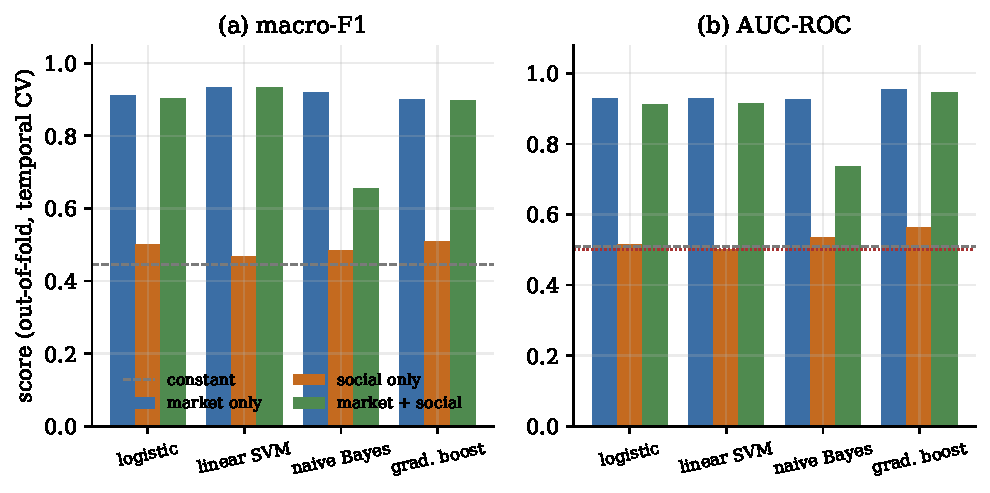
\includegraphics[width=\linewidth]{fig_task3_models.pdf}
\caption{Task-3 temporal-CV ablation. (a)~macro-F1 and (b)~AUC-ROC for each model family,
grouped by feature set (market only / social only / market\,+\,social). The market arm
(blue) dominates across every family; the social arm (orange) sits at the constant
baseline (grey dashed) and the chance line (red dotted); adding social to market (green)
yields no consistent gain.}
\label{fig:task3}
\end{figure}

\section{Complementary view: final pre-close backtest}
As a calibration-focused cross-check we also keep the Branch-09 single-cut backtest --- one
final pre-close prediction per contract, scored under 5-fold out-of-fold cross-validation
(\Cref{tab:results}, \Cref{fig:models}). It tells the same story from the probabilistic
angle: market-only attains Brier $0.031$ / AUC $0.989$, while market+social is slightly
\emph{worse} and social-only is below chance (AUC $0.404$).

\begin{table}[H]
\centering
\caption[Final pre-close backtest over 300 resolved contracts]{Final pre-close backtest
(5-fold out-of-fold; lower Brier/log loss, higher accuracy/AUC are better). The best
probabilistic score in each column is bold.}
\label{tab:results}
\small
\setlength{\tabcolsep}{5.5pt}
\begin{tabular}{@{}l r r r r r@{}}
\toprule
\textbf{Model} & \textbf{Brier}$\downarrow$ & \textbf{Log loss}$\downarrow$ &
\textbf{Accuracy}$\uparrow$ & \textbf{AUC}$\uparrow$ & \textbf{ECE}$\downarrow$\\
\midrule
base rate      & 0.154 & 0.486 & 0.810 & 0.487 & \textbf{0.003}\\
\rowcolor{pslight} market-only    & \textbf{0.031} & \textbf{0.110} & \textbf{0.963} & \textbf{0.989} & 0.020\\
social-only    & 0.160 & 0.504 & 0.810 & 0.404 & 0.060\\
market + social& 0.040 & 0.187 & 0.963 & 0.975 & 0.091\\
\midrule
\multicolumn{6}{@{}l}{\footnotesize\itshape Lift of market+social over market-only:\;
$\Delta\text{Brier}=-0.009$,\; $\Delta\text{LogLoss}=-0.077$ (both negative $=$ worse).}\\
\bottomrule
\end{tabular}
\end{table}

\begin{figure}[H]
\centering
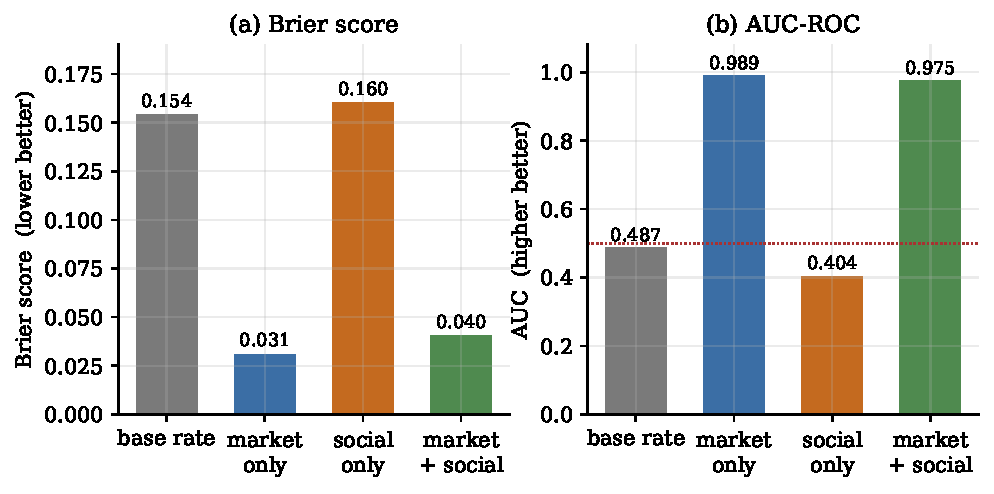
\includegraphics[width=\linewidth]{fig_model_comparison.pdf}
\caption{Final pre-close model comparison. (a)~Brier score and (b)~AUC. The market-only
baseline (blue) is the best model; adding social features (green) degrades it, and
social-only (orange) is no better than the chance line.}
\label{fig:models}
\end{figure}

\paragraph{Calibration.} \Cref{fig:calibration} shows the reliability of the two
price-based models. Market-only is well calibrated (ECE $0.020$): its predicted
probabilities match observed outcome frequencies closely, in the sense
of~\cite{niculescu2005predicting}. Market+social is visibly
\emph{less} calibrated (ECE $0.091$) --- the noisy social features push some
predictions away from the well-calibrated price.

\begin{figure}[H]
\centering
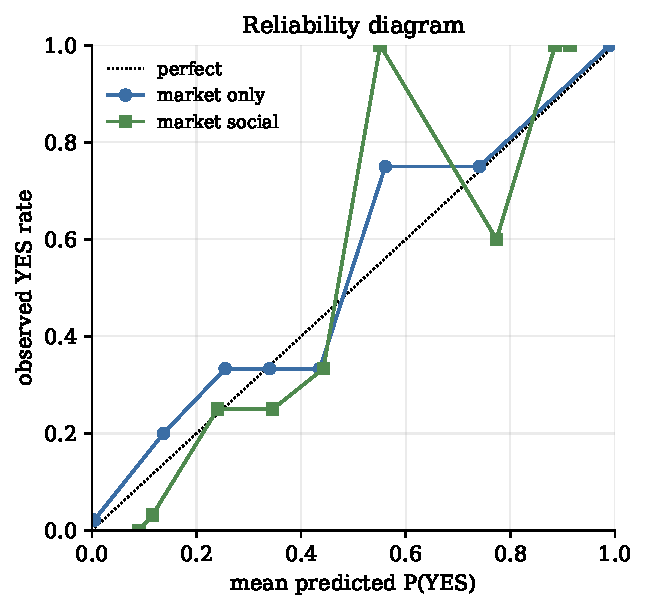
\includegraphics[width=0.5\linewidth]{fig_calibration.pdf}
\caption{Reliability diagram. The market-only model (blue) hugs the diagonal; adding
social features (green) worsens calibration.}
\label{fig:calibration}
\end{figure}

\paragraph{Why the combined model does not improve.} The fitted coefficients
(\Cref{fig:features}) tell the story compactly: the market-probability coefficient
($1.68$) dwarfs every social coefficient (all $|\beta|<0.10$). The model learns to trust
the price and to all but ignore the social features --- and the small weight it does put
on them adds variance, not signal.

\begin{figure}[H]
\centering
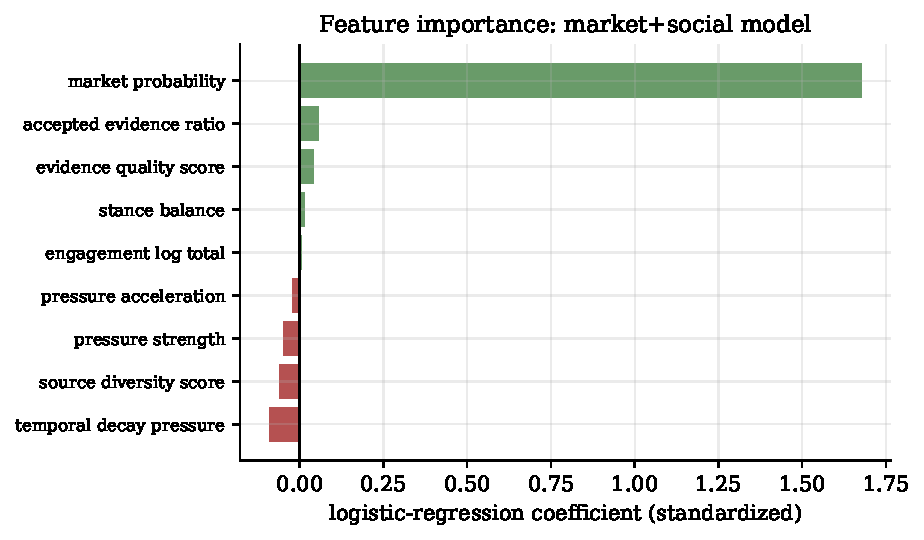
\includegraphics[width=0.72\linewidth]{fig_feature_importance.pdf}
\caption{Standardised logistic-regression coefficients of the market+social model. The
market probability dominates; the social features carry negligible, mixed-sign weight.}
\label{fig:features}
\end{figure}

\section{Does more evidence help? A coverage ablation}
A natural objection is that the social signal fails only because coverage is thin. We
test this by restricting the social-only model to the 73 contracts with
\emph{sufficient} accepted evidence. It does not rescue the signal: even there the model
predicts \textsc{No} for every contract, so its nominal AUC of $0.56$ reflects ranking
noise on an all-\textsc{No} classifier rather than usable signal; on the 227
insufficient-evidence contracts the AUC is $0.35$. The aggregate stance--outcome
correlation is $-0.015$ and the engagement-weighted net-pressure--outcome correlation is
$-0.013$ --- both indistinguishable from zero. \textbf{Within the range of coverage we have, more evidence
does not convert into predictive value}; the problem is the nature of the signal, not
merely its quantity (we revisit the quantity question, honestly, in
\Cref{ch:limitations}).

\begin{takeaway}
\textbf{Headline result.} Under expanding-window temporal cross-validation, all four
model families place the market arm at macro-F1 $0.90$--$0.93$ / AUC $0.93$--$0.95$,
while the social-only arm sits at near-chance macro-F1 $0.47$--$0.51$ (AUC $\approx0.5$)
and combining the two yields no consistent gain. The final pre-close backtest agrees:
market-only scores Brier $0.031$ / AUC $0.989$, adding social makes it \emph{worse}, and
social-only is below chance (AUC $0.404$). Social discourse adds \emph{no} incremental
predictive value over the Polymarket price in this dataset.
\end{takeaway}


%==============================================================================
\chapter{Discussion}
\label{ch:discussion}

The predictive result is negative and robust. This chapter explains \emph{why}, and
argues that the finding is informative rather than disappointing.

\section{Three structural causes}
\paragraph{1. The market is already efficient with respect to public information.}
By the efficiency argument of \Cref{ch:background}, any genuinely predictive public
signal tends to be arbitraged into the price. \Cref{sec:informative} quantified just how
strong that price already is --- AUC $0.90$ a full quarter before resolution. A public,
lagging social signal has essentially no room left to add value; the only edge would
come from \emph{private} or \emph{early} information, which broadcast Telegram channels
and public Reddit threads do not carry.

\paragraph{2. Social discourse is optimism-biased.}
Stance leans \textsc{Yes} $2.3{:}1$ while contracts resolve \textsc{No} $4.3{:}1$
(\Cref{fig:stance}), and on 58 of the 72 contracts where social pressure says
\textsc{Yes} the market resolves \textsc{No} (\Cref{fig:hype}). Discourse concentrates on
the exciting possibility that an event \emph{will} happen; markets, pricing base rates,
know that most such events do not. A signal that is systematically wrong in direction
cannot help a calibrated forecaster.

\paragraph{3. The discourse is reactive, not leading.}
The lead--lag analysis (\Cref{ch:correlation}) found no horizon at which social changes
precede price changes. Social media here narrates events the market has already priced; many candidate posts were
rejected by the temporal-admissibility filter for falling \emph{after} a contract had
already closed. A coincident-or-lagging signal cannot improve a forecast made before the
event.

\section{A note on coverage}
A fourth factor --- the channel/market mismatch (\Cref{ch:crossplatform}) --- limits how
much of the market the social layer even \emph{covers}: politics absorbs 81\% of
evidence, sports almost none. Crucially, though, the coverage ablation
(\Cref{sec:results}) shows that the failure is not merely one of quantity: even where
evidence is dense, its direction does not track outcomes. Broader coverage would let us
test more contracts, but on present evidence there is no reason to expect it to overturn
the direction of the result.

\section{Why a null result matters}
This is not a failed experiment; it is a clean, reproducible piece of evidence in a
literature crowded with fragile positive claims. It (i)~empirically corroborates the
informational efficiency of a major prediction market against a large, realistic social
corpus; (ii)~demonstrates a methodology --- leakage controls, ablation, calibration ---
that distinguishes genuine incremental value from spurious correlation; and (iii)~maps
precisely \emph{where} a social edge would have to come from (private/early signals,
information-asymmetric events) for future work to find it. ``PolySignal does not beat
Polymarket'' is, in this framing, exactly the finding.


%==============================================================================
\chapter{Limitations and Future Work}
\label{ch:limitations}

\section{Limitations}
We state the limitations plainly, since several of them bound the strength of the
conclusion.
\begin{description}[leftmargin=1.4em,style=nextline]
  \item[Platform coverage.] All three platforms are present in the analysed corpus, but
  it is \textbf{Telegram-dominated} (98.6\%), with a secondary Reddit contribution
  (1.2\%) and a small X/Twitter sample (0.2\%) whose scale is capped by X's
  anti-automation defences (\Cref{sec:scope}). The 68 Telegram channels are a purposive,
  not a random, sample, with a clear crypto/macro/geopolitics tilt. The predictive
  conclusions therefore hold for a Telegram-dominated corpus skewed towards
  crypto-adjacent discourse; whether a \emph{volume-balanced} three-platform corpus would
  change them is the central open question, and the architecture is built to answer it
  without code changes once such a corpus is available.
  \item[Domain coverage.] Sports contracts have almost no social evidence; the
  predictive conclusion is therefore strongest for politics and finance and weakest for
  sports.
  \item[Comments and authors.] Only a bounded \emph{sample} of per-comment text is
  collected, so comment-derived
  features are thin; broadcast Telegram channels expose neither follower counts nor
  author profile URLs, so those required fields are partially empty for that platform.
  \item[Deterministic baselines.] Linking and stance use deterministic heuristics; the
  optional cached LLM verifiers were not run at scale, which leaves $73\%$ of stance
  rows \code{neutral} and the heuristic NER noisy.
  \item[One prediction per contract.] Although we now score under expanding-window
  temporal cross-validation across contracts, each contract still contributes a single
  pre-close prediction; intra-contract time-sliced 7/3/1-day forecasts are deferred until
  the price/feature history is broad enough to support them cleanly.
  \item[Binary contracts only.] Multi-outcome markets are out of scope.
\end{description}

\section{Future work}
The limitations map directly to next steps, ordered by expected payoff:
\begin{enumerate}
  \item \textbf{Close the coverage gap.} Broaden the X/Twitter and Reddit passes (e.g.\
  via a paid research tier) and add sports-specific channels, so that all three platforms
  and all three domains carry \emph{comparable} evidence --- turning the cross-platform
  layer of \Cref{ch:crossplatform} into a volume-balanced three-platform complementarity
  test (Task~2.4).
  \item \textbf{Stronger stance and linking.} Run the cached LLM stance/relevance
  judges at scale and adopt the spaCy NER backend, reducing the neutral mass and the
  entity noise.
  \item \textbf{Time-sliced and early-signal evaluation.} Score 7/3/1-day pre-close
  windows and explicitly search for contracts where social \emph{leads} the price ---
  the only regime in which an edge is theoretically possible.
\end{enumerate}


%==============================================================================
\chapter{Conclusions}
\label{ch:conclusions}

We set out to determine whether social-media discourse adds predictive value over
Polymarket's own prices. To answer it we built an end-to-end Big Data pipeline that
collects 300 resolved binary contracts and their full-lifetime price series
($1{,}353{,}114$ points), collects a longitudinal multi-platform corpus
($1{,}368{,}041$ posts across Telegram, Reddit, and a small X/Twitter sample,
\Cref{sec:scope}), links posts to contracts with a deterministic semantic scorer,
enriches the text
with sentiment, entities, topics, and outcome-aware stance, projects everything into a
Neo4j knowledge graph, and condenses the evidence into a per-market Social Pressure
Index that feeds a leakage-controlled backtest --- all exposed through an interactive
dashboard. The system satisfies each requirement of Tasks~1, 2, and the optional
Task~3.

The descriptive study confirmed that Polymarket prices are already highly informative of
outcomes and become more so as resolution nears (AUC $0.90\!\to\!0.99$). The predictive
study returned a clear, well-controlled \textbf{null result} that is robust across four
model families under expanding-window temporal cross-validation: the market arm reaches
macro-F1 $0.90$--$0.93$ and AUC up to $0.95$, the social-only arm never escapes
near-chance (macro-F1 $\approx0.5$), and combining the two adds no consistent lift; the
final pre-close backtest concurs (market-only Brier $0.031$ / AUC $0.989$, market+social
\emph{worse}, social-only below chance). We traced this to the market's informational
efficiency, a systematic optimism bias in
social stance, the reactive (non-leading) nature of the discourse, and a structural
mismatch between the available channels and the contract sample.

The contribution of this work is therefore twofold: a reproducible, leakage-aware
methodology for studying social signals against prediction markets at scale, and the
honest empirical finding that public social discourse does not, in this setting, beat
the market price. In a field prone to over-claiming, demonstrating \emph{where} and
\emph{why} a signal fails --- and doing so reproducibly --- is a result worth reporting.
